
%sudo apt-get install texlive-bibtex-extra
%Word counts: pdftotext WBVFM_IntroPar.pdf - | wc -w
\documentclass{article}\usepackage[]{graphicx}\usepackage[]{color}
%% maxwidth is the original width if it is less than linewidth
%% otherwise use linewidth (to make sure the graphics do not exceed the margin)
\makeatletter
\def\maxwidth{ %
  \ifdim\Gin@nat@width>\linewidth
    \linewidth
  \else
    \Gin@nat@width
  \fi
}
\makeatother

\usepackage{Sweave}


\usepackage{float}
\usepackage{wrapfig}
\usepackage{hyperref}
\usepackage{authblk}
\usepackage{tablefootnote}
\usepackage[backend=bibtex, style=nature, citestyle=authoryear]{biblatex}
\bibliography{WBVFM_IntroPar}
\newenvironment{knitrout}{}{}  %just a dummy environment
\makeatletter
\newcommand\gobblepars{%
    \@ifnextchar\par%
        {\expandafter\gobblepars\@gobble}%
        {}}
\makeatother



\author[1]{Daniel Runfola\thanks{dsmillerrunfol@wm.edu}}
\author[1]{Ariel BenYishay\thanks{abenyishay@wm.edu}}
\author[2]{Jeff Tanner\thanks{jtanner@worldbank.org}}
\author[3]{Graeme Buchanan\thanks{graeme.buchanan@rspb.org.uk}}
\author[4]{Jyothy Nagol\thanks{jnagol@umd.edu}}
\author[5]{Matthias Leu\thanks{mleu@wm.edu}}
\author[1]{Seth Goodman \thanks{smgoodman@wm.edu}}
\author[1]{Rachel Trichler\thanks{rbtrichler@wm.edu}}
\author[1]{Rob Marty\thanks{ramarty@email.wm.edu}}

\affil[1]{Institute for the Theory and Practice of International Relations, The College of William and Mary}
\affil[2]{Independent Evaluation Group, World Bank}
\affil[3]{Center for Conservation Science, Royal Society of Birds}
\affil[4]{Global Land Cover Facility, University of Maryland}
\affil[5]{Department of Biology, The College of William and Mary}

\renewcommand\Authands{ and }

\title{A top-down approach to estimating spatially hetereogeneous impacts of development aid on vegetative carbon sequestration}
\date{\vspace{-5ex}}
\IfFileExists{upquote.sty}{\usepackage{upquote}}{}
\begin{document}
\begin{knitrout}


\maketitle 
\begin{flushleft}
\textbf{Short Title}: Estimating impacts of aid on carbon sequestration\\
\textbf{Keywords}: International Aid, Carbon Sequestration, Causal Identification, Heterogeneous Effects\\
\textbf{Words in Abstract:} 150\\
\textbf{Words in Manuscript:} 3000\\
\textbf{Number of References:} 30\\
\textbf{Number of Figures and Tables:} 10\\
\textbf{Corresponding Author}:\\
Dr. Daniel Runfola\\
Institute for the Theory and Practice of International Relations, \emph{AidData}
Email: dsmillerrunfol@wm.edu
Telephone: 508.316.9109
Fax: 757.221.4650
\end{flushleft}

\newpage
\section{Abstract}
  Since 1945, over \$4.9 trillion dollars of international aid has been allocated (\cite{tierney_more_2011}).
 To date there have been no estimates of the regional impact of this aid on the carbon cycle.  
 We apply a geographically explicit matching method (\cite{andam_measuring_2008}) to estimate the impact of World Bank projects implemented between 2000 and 2010 on sequestered carbon, using a novel and publically available dataset of 47,084 World Bank project locations. 
 Considering only carbon sequestered due to fluctuations in vegetative biomass caused by World Bank projects, we estimate a global net positive increase in sequestration totaling 1,398,229 tonnes. 
However, we illustrate the apparent effectiveness of environmental safeguards (\cite{laurance_reducing_2015}) implemented by the World Bank are variable across different geographic contexts.  
We argue that subnational data can be helpful in the identification of these heterogeneous impact effects, and highlight the considerable methodologic barriers which still exist.

\newpage
\section{Introduction}
International recognition of the dual challenges of international development and the mitigation of environmental change is resulting in a large redirection of resources towards developing countries. 
The United States alone has pledged nearly \$4 billion dollars of aid to mitigate climate vulnerability over the next 4 years, and the Paris convention urged donors to target \$100 billion annually by the year 2020 (\cite{royal_united_2015}). 
Coupled with increasing pressure from recipient nations, donors have and continue to introduce more stringent environmental safeguards, including requirements for compliance with national and international regulations, environmental management plans, reforestation goals, and others (\cite{nielson_delegation_2003}, \cite{gutner_explaining_2005}).
\par
Despite these shifts in the policies of donor agencies, there is a gap in empirical studies examining the impacts of these policies on environmental outcomes.  
This letter aims to illustrate an approach to overcoming this gap, as well as highlight many of the remaining methodological challenges.
We specifically examine the impact of World Bank projects on vegetation and subsequent changes in carbon sequestration, leveraging a novel and publically available dataset of 47,084 World Bank project locations \footnote{http://aiddata.org/level1/geocoded/worldbank} in conjunction with long-term satellite data quantifying vegetative biomass and a number of spatially-referenced control variables (see table \ref{data_source_table}),

\begin{table}

\begin{tabular}[h]{|p{4.5cm}||p{7cm}|}
\hline
\multicolumn{2}{|c|}{\texttt{Data Sources}} \\
\hline
\textbf{Data Name} & \textbf{Source} \\
\hline
Gridded Population of the World & Center for International Earth Science Information Network\tablefootnote{http://sedac.ciesin.columbia.edu/data/collection/gpw-v3/sets/browse} \\
\hline
Nighttime Lights & Defense Meteorological Satellite Program\tablefootnote{Stable Lights retrieved from http://ngdc.noaa.gov/eog/dmsp.html}\\
\hline
Precipitation and Temperature & University of Delaware (\cite{willmott_terrestrial_2001})\tablefootnote{Variables derived from these product included the average precipitation (P) and temperature (T) before a project was implemented (from 1992), the linear trend in P and T from 1992 to the project impelmentation, the average temperature from the date the project was implemented until the end of the temporal record(2012), and the post-project trend through 2012. Absolute measurements of each variable were also retained. } \\
\hline
Urban Travel Time & European Commission Joint Research Centre\tablefootnote{http://forobs.jrc.ec.europa.eu/products/gam/download.php}\\
\hline
Distance to Rivers & World Wildlife Fund \tablefootnote{http://hydrosheds.cr.usgs.gov/index.php}\\
\hline
Vegetation & NASA LTDR\tablefootnote{http://ltdr.nascom.nasa.gov/cgi-bin/ltdr/ltdrPage.cgi} \\
\hline
Carbon Storage & NASA JPL (\cite{saatchi_benchmark_2011})\tablefootnote{http://click.jpl.nasa.gov/Archive/carbon/ftpdata/carbon/datasets/} \\
\hline
Ecofloristic Zone Carbon Fractions & Oak Ridge National Laboratory (\cite{ruesch_new_2008}) \\
\hline
\end{tabular}
\caption{Data sources used in this analysis.}\label{data_source_table}
\end{table}

\par
We find that while the overall impact of World Bank projects on carbon sequestration appears to be positive (an increase of 1,398,229 sequestered tonnes), considerable temporal and spatial variation exists in these impacts
Further, we illustrate the advantages and limitations of a geographically explicit approach to estimating the causal effects of development aid projects, and outline a number of topics for further research.
Finally, we introduce an enhanced, publically available dataset of the global, spatially-explicit distribution of World Bank activities encompassing projects initiated between 1995 and 2014.


\section{Methods}
Over the last five years, significant progress has been made on methods which integrate spatial data (i.e., satellite information on forest cover) to quantify the causal impact of interventions (i.e., projects aimed at the prevention of deforestation) (\cite{buntaine_titling_2015};\cite{nelson_effectiveness_2011}).  
These methods largely rely on propensity score and other matching-based methods to select "control" cases where no or limited intervention occured, and match these with similar "treatment" cases (\cite{andam_measuring_2008}). 
We build on these approaches, implementing a geographically explicit two-stage Propensity Score Matching estimation strategy. 
\subsection{Geographically Explicit Impacts}
First, we truncate the dataset to cover World Bank projects from 2000 to 2010 due to limitations of our ancillary information, resulting in a total of 47,084 World Bank project locations.
Second, the area of influence within which we anticipate each World Bank project could plausibly have an impact on deforestation is calculated by examining the historic spatial distance at which forest cover is spatially correlated before any projects were implemented. To parameterize this distance, we calculate a Moran’s I (\cite{getis_the_1992}) score at increasing distances, identifying the distance at which spatial autocorrelation is no longer predominant for our outcome measure of forest cover, measured in 1999.  
We argue that this estimate is a highly conservative estimate of the possible area of influence a project could have (i.e., we will tend to over-estimate the buffer size), as it represents the totality of historic spillovers up to the year 1999.
\par
For each of 12 distance bins (between 0 and 2,200 kilometers, in increments of approximately 180km), Moran’s I is calculated following:

\begin{equation}
I_h = (\frac{N}{\sum_{i}^{N}\sum_{j}^{N}w_{ij}}) * ((\sum_{i}^{N}\sum_{j}^{N}w_{ij} * (X_{i}-\bar{x}) * \frac{X_{j} - \bar{x}}{\sum_{i}^{N}(X_{i}-\bar{x})})^{2})
\end{equation}
where \textit{h} represents each spatial bin, \textit{N} the number of spatial units, \textit{i} and \textit{j} are indexes for each unit, \textit{X} is the variable of itnerest, and \begin{math}W_{ij}\end{math} represents the weights matrix.  
In this application, the weights matrix is specified according to the bin (\textit{h}) being analyzed.  
\par
Once calculated, the distance at which Moran's I is equal to or less than .10 is identified, and used to parameterize a buffer around each project.  
The projects are then subdivided into six different project (sector) types - Health, Environment, Education, Industrial, Infrastructure, and Other.  
Within each of these sectors, projects are further subdivided into three equally-sized monetary bins of "low", "medium", and "high" dollars commited to the project.
\par
Finally, for each sector-monetary bin combination (18 total groups), a geographically explicit propensity score model is fit.  
This is conducted following a three-stage process which is repeated for every unit of analysis, resulting in 47,084 total model estimations.
In the first stage, a unit of observation is selected and all World Bank projects that fall within the distance estimated according to the Moran's I are selected as the relevant "sub population" for that point.
All points within the sub-population are defined as treated or untreated pending the monetary value being analyzed - for example, if the unit of observation selected is a high dollar value project, all projects in the medium and low bins are assigned an untreated value (0), while all high dollar value projects are assigned as treated (1).
\par
In the second stage, all points within the sub-population are matched according to a propensity score matching routine.  Variables matched on can be seen in Table 1, and matches were limited to be within the same sector. The propensity scores are calculated following:
\begin{equation}
T = \beta_{0} + \sum_{k=1}^{k}(\beta_{k}*x_{k})
\end{equation}
where \textit{T} is the treatment binary, and \begin{math}\beta_{k}\end{math} are the estimated coefficients for each covariate, \begin{math}x_{k}\end{math}.  
The estimates from this equation are applied to each unit of observation within the sub-population, and the differences between propensity scores across different units of observation represent a univariate measure of similarity.  
For the set of treated units within the area of influence, the optimal set of matched untreated units was identified using a nearest-neighbor optimization \cite{ho_matchit:_2011}. \par
In the third stage, a regression relationship is calibrated between the outcome measure (The average LTDR NDVI value in the years after project implementation), the treatment binary, and all available covariates:
\begin{equation}
y_i = \beta_{0} + \beta_{1} * T + \sum_{k=1}^{k}(\beta_{k}*x_{k}) + D_{p}
\end{equation}
where \begin{math}y_{i}\end{math} represents the level of forest cover within each zone \textit{i}, \begin{math}\beta_{1}\end{math} represents the estimated impact of the treatment, and \begin{math}and D_{p}\end{math} represent fixed effects for each paired observation.
Every unit of observation \textit{n} has a zone \textit{i}, defined as all projects which fall within the distance calculated using Moran's I.
\par
This three-step process is repeated for every unit of observaiton.  
In some cases, insufficient matches or eligible cases existed to approximate the impact for a region; these units were omitted from the analysis.

\subsection{Estimating Carbon Sequestration}
Because the outcome measure examined (NDVI) is only a proxy for tree cover, an additional step of modeling must be conducted to translate changes in NDVI into changes in estimated tonnes of carbon sequestered.



\section{Results}
The Results section should present the experiments that support the conclusions to be drawn later in the Discussion. The Results section should conform to a high standard of rigour. Extended lines of inference, arguments or speculations should not be placed in the Results.

\begin{wrapfigure}[20]{r}{0.65\textwidth}\centering
%\begin{minipage}{.75\textwidth}
\begin{Schunk}

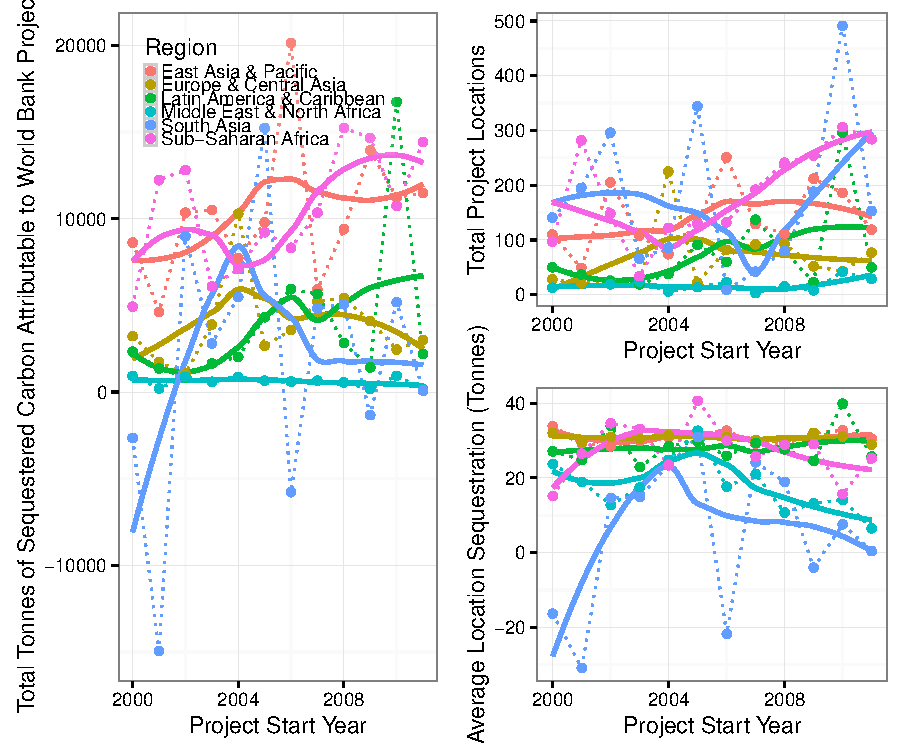
\includegraphics[width=\maxwidth]{figure/Fig1-1} \end{Schunk}
%\end{minipage}
\end{wrapfigure}  

\section{Discussion}
This approach has the benefit of comparing "apples to apples" - i.e., World Bank project locations are contrasted to others at which it is known a World Bank project exists.
However, it also has the disadvantage of limiting the eligible set of matches to locations at which World Bank projects are.

The Discussion section should be separate from the Results section. It allows authors to propose their interpretation of the results, and to suggest what they mean in a wider context. It should end with a clear statement of the main conclusions of the research, and a clear explanation of their importance and relevance to applied conservation and/or policy.

\section{Acknowledgements}
The authors would like to acknowledge the government of Sweden and the World Bank Independent Evaluation Group for partially funding this research.  This work was performed in part using computational facilities at the College of William and Mary which were provided with the assistance of the National Science Foundation, Virginia Port Authority, Virginia's Commonwealth Technology Research Fund, and the Office of Naval Research.  The authors would also like to thank Scott Stewart, Alex Kappel, Miranda Lv, Doug Nicholson, and Vinay Vijayan for their valuable contributions and insights.


\newpage
\section{References}
%Need to ensure formatting is correct -
%http://endnote.com/downloads/style/conservation-letters
%Limited to 40 references
\printbibliography



\end{knitrout}
\end{document}
